\chapter{Bullet Rectangle Bounding Box}\label{cha:meth}
For this thesis a comparative evaluation was decided upon, for that a baseline is
required. I decided on a rectangle bounding box around the model
as a simple method to compare against. It has obvious shortcomings in all
areas, except maybe, performance.

\section{Implementation}\label{sec:recImpl}
An axis-aligned bounding rectangle is fitted around the model.
Bullet includes a collision shape for rectangles and these rectangles can be used
to represent the ground plane and the bin itself, i.e. the world.

Bullet 2.83 is used to simulate the rigid body system.
Bullet's sequential impulse solver is used to simulate the system. The broadphase
was set to AxisSweep3, with a simulation world as large as the bin, with some margin, in the
xz plane and thrice the height of the bin for y, as the models are initiated in a stack
above the bin. This height could easily be calculated and set to fit snuggly instead.
However, using the same world size for each simulation gives more comparable time measurements.

In figure~\ref{fig:startStack} the initial distribution of the models is visualized.
The models are placed in a stack spaced as to not intersect, and shifted with a random
offset in the xz-plane to inject some chaotic behavior in the final distribution.
The final state of this simulation is visualized in figure~\ref{fig:stopStack}
without bounding boxes rendered and with bounding boxes rendered in figure~\ref{fig:stopStackBoxes}.

\begin{figure}[H]
  \centering
  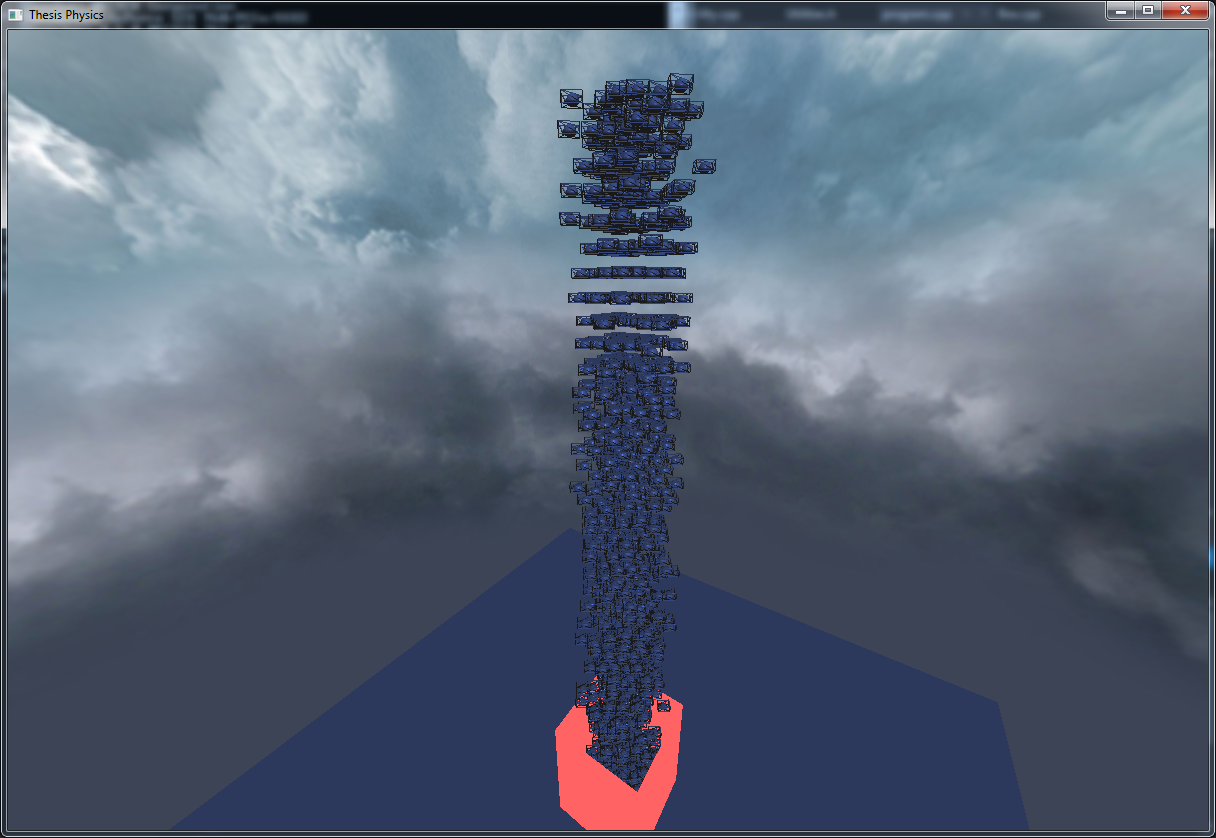
\includegraphics[width = 0.8\textwidth]{Screenshots/startofSimulation1000bodies01-22(Bugged).png}
  \caption{The start state of the simulation. Models are stacked with some margin in between and translated by a offset in the xz plane randomly. }
  \label{fig:startStack}
\end{figure}

\begin{figure}[H]
  \centering
  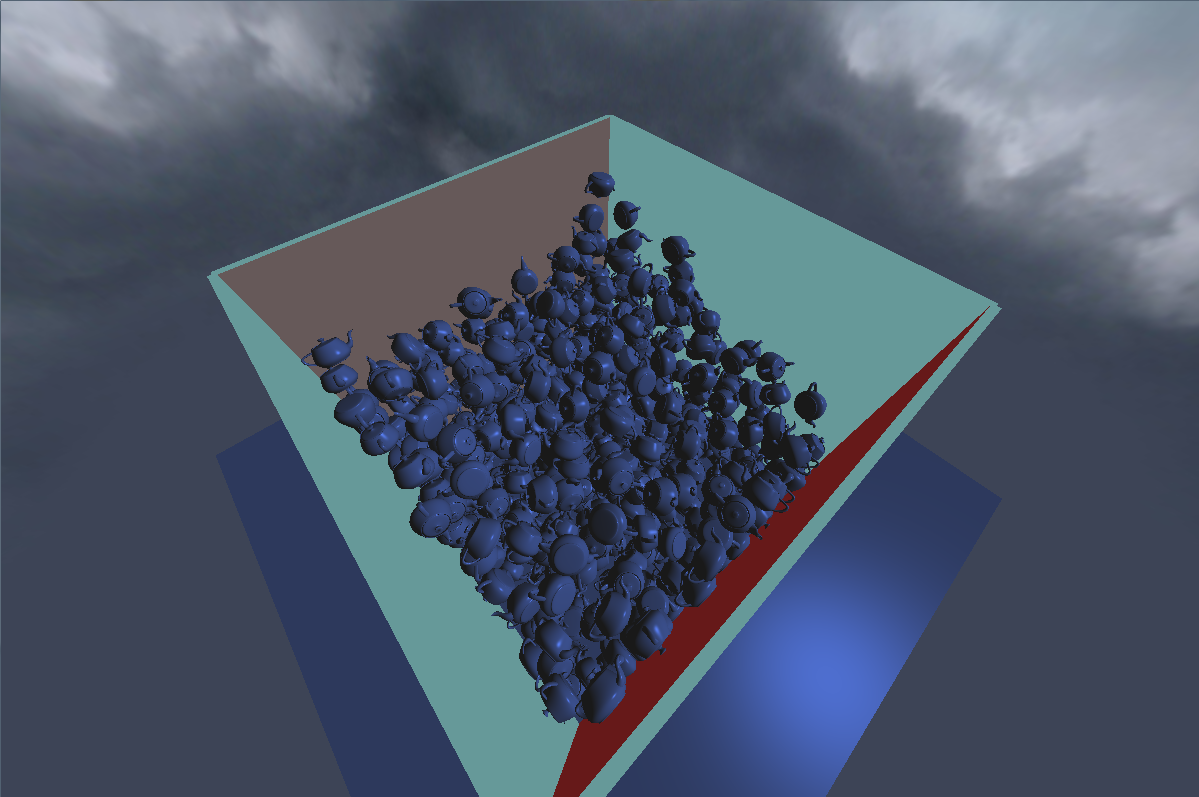
\includegraphics[width = 0.8\textwidth]{boxesNoBox04-22.png}
  \caption{The final state of the simulation.}
  \label{fig:stopStack}
\end{figure}

\begin{figure}[H]
  \centering
  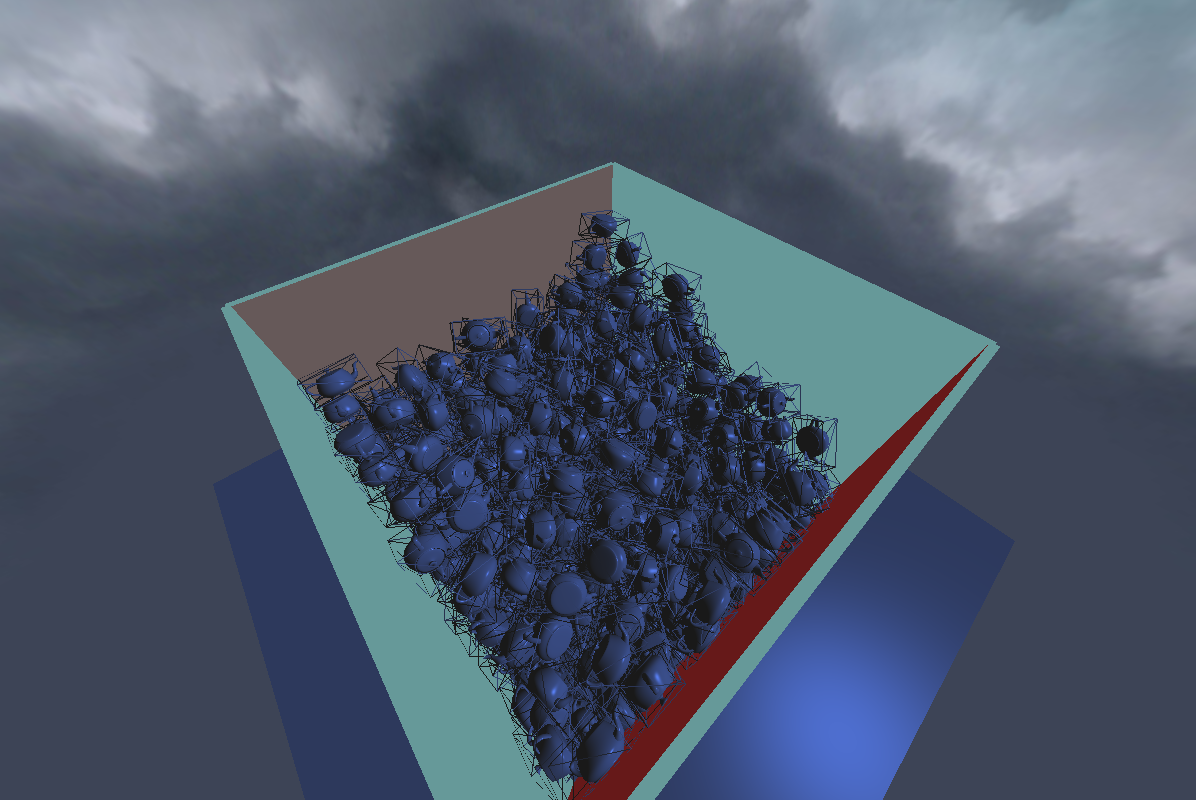
\includegraphics[width = 0.8\textwidth]{boxes04-22.png}
  \caption{The final state of the simulations with bounding boxes drawn.}
  \label{fig:stopStackBoxes}
\end{figure}

\section{Testing}\label{sec:testing}
Different parameters were tested to see how they affect the system in terms of performance.
The different parameters get their own explanation below, the full test data can be found in appendix~\ref{app:bullet}.
The figures present total simulation time with respect to energy threshold and sub-iterations used and
frame times for the same parameters. In addition differently sized objects were tested
as the number of layers in the stacking greatly affect the simulation time.

For details on the relaxation used see subsection~\ref{subsec:relax}.
All of the testing is done with a fixed time step of 1/60 seconds. Using a less detailed
time step lead to some of the parameter constellations to never converge.
The tests were all seeded with the the same initial seed for the random generator,
as to reproduce the initial state.

\subsection{Energy Treshold}\label{subsec:relax}
Most of the simulation time happens at the end of the simulation and only small
adjustments are made. This is not surprising at all. Basically when all objects
fall into the bin they can interpenetrate somewhat and most are not in
a stationary state. When the object then moves almost the whole system receive
repercussions of that movement. These new movements shift more objects and the
system might oscillate for a while before it finally comes to rest.
Bullet puts objects to sleep when their angular and linear velocities reach certain
thresholds, these thresholds can be modified or we can
allow the system to finish early. In this implementation I skip Bullets sleeping
thresholds and directly measure the energy of the bodies and relax the system by
allowing the system to end a simulation when the system reaches a certain
average energy per body threshold. This threshold significantly increases the performance
of the system as the small adjustments at the end tend to oscillate quite a lot before
stabilizing out completely.

\begin{equation}
E_{avg} = \frac{1}{N}\sum_{i=0}^{N-1}E_i
\end{equation}

When the system is allowed to run to zero energy, Bullets sleeping thresholds are
used. Note that at a energy threshold of 0.1 J I have never been able
to find a visual discrepancy in the distribution of the parts. Bullet inserts an
artificial additional gap between object of 0.04 units (for collision detection purposes).
So ending the simulation somewhat early is quite safe. Setting this energy threshold
too high will give obvious issues.

\subsection{Sub iterations}
The Sequential Impulse solver uses sub-iterations to resolve interpenetrations within
a time step. The amount of sub-steps taken can influence performance and how detailed
the solution is. Erwin Coumans recommends this parameter to be set between 4 and 10. Coumans E.[2015]

\subsection{Prescale factor}
The scale factor used on the model before the system is simulated.
Smaller models act more and more as a liquid where small changes propagate further
and further since less unoccupied space exist.

\subsection{Iterations}
How many iterations it took for the system to come to rest. The system is always
advanced in steps of 100 iterations since the energy needs to be measured and it
is, while quite cheap, affecting the time measurements. By only measuring intermittently
their influence on the time is reduced.

\subsection{Time}
Total time in milliseconds the simulation took, including the energy measurement
every 100 iterations.

\subsection{End energy}\label{subsec:enden}
If a threshold greater than 0 is used there will be some residual energy left in the
system.

\section{Results}
\subsection{Prescale 0.5}
The following timings are using a prescale of 0.5. The model is reduced in size by
half in each dimension before simulation. As these measurement as relative one could
theoretically made the bin larger instead. However the important point here is when reviewing the
next test series that test series uses models half as large as this test series.
\begin{figure}[H]
  \centering
  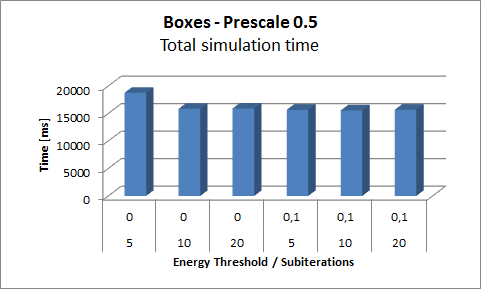
\includegraphics[width = 0.8\textwidth]{graphs/totalTimeBoxes05.png}
  \caption{The influence of energy threshold and subiterations on total simulation time.}
  \label{fig:totalTimeBoxes05}
\end{figure}

\begin{figure}[H]
  \centering
  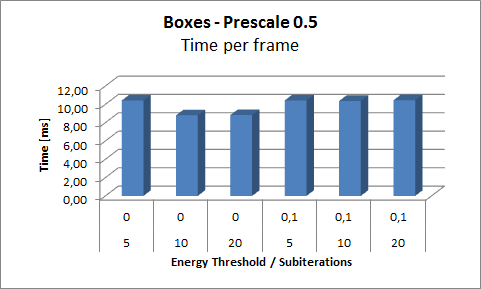
\includegraphics[width = 0.8\textwidth]{graphs/frameTimeBoxes05.png}
  \caption{The influence of energy threshold and subiterations on time per frame.}
  \label{fig:frameTimeBoxes05}
\end{figure}

\subsection{Prescale 0.25}
As previously noted, the models here are half as large in each dimension in comparison to
the previous time series, where the prescale was set to 0.5.
\begin{figure}[H]
  \centering
  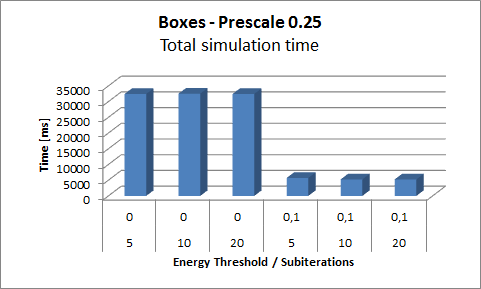
\includegraphics[width = 0.8\textwidth]{graphs/totalTimeBoxes025.png}
  \caption{The influence of energy threshold and subiterations on total simulation time.}
  \label{fig:totalTimeBoxes025}
\end{figure}

\begin{figure}[H]
  \centering
  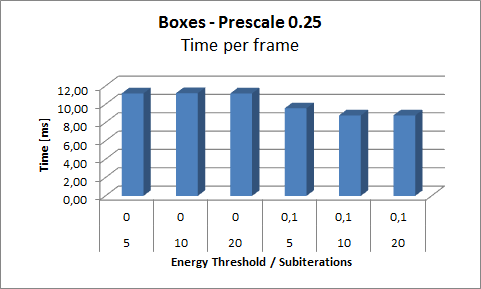
\includegraphics[width = 0.8\textwidth]{graphs/frameTimeBoxes025.png}
  \caption{The influence of energy threshold and subiterations on time per frame.}
  \label{fig:frameTimeBoxes025}
\end{figure}

An example of the end state of the simulation is given in the figure below.
\begin{figure}[H]
  \centering
  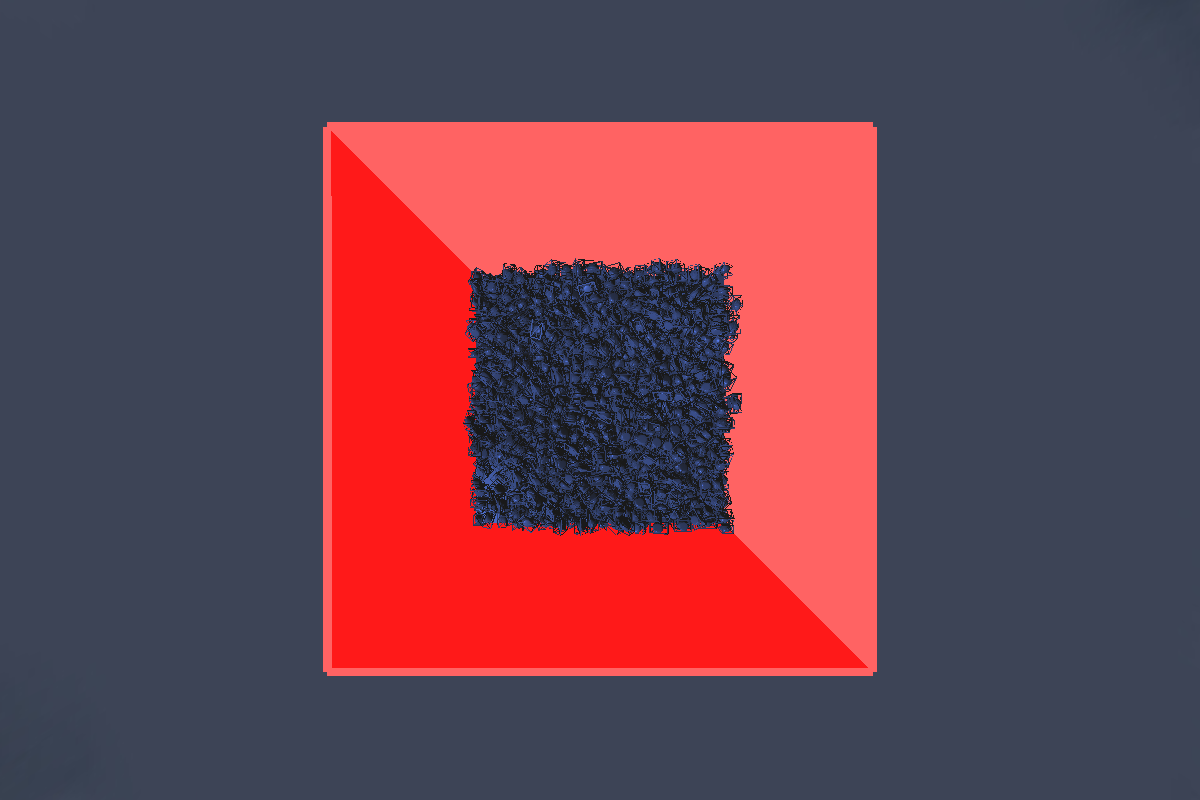
\includegraphics[width = 0.8\textwidth]{Screenshots/endState025.png}
  \caption{Finished simulation}
  \label{fig:endstate}
\end{figure}

\newpage
\subsection{Remarks}
The energy threshold saves a lot of simulation time for when the objects are small.
Small movements of a single object result in long chains of movement and the whole
system spends a lot of time adjusting at the end of the simulation state. The overall
motion at the end is small and no major adjustments are made. The early energy exit
strategy give good performance increases with small sacrifices to overall correctness
of the end state. We do not see a large performance increase for the larger models,
but the feature can, if wanted, be left activated for those scenarios as well.

The amount of sub-iterations do not seem to have a huge impact on neither simulation
quality nor simulation time.
During testing it has however been noted that selecting a very low amount of
sub-iterations, for example one iteration, could in some cases lead to oscillating,
 non-stabilizing systems. These observations let me decide on a fixed amount of sub-iterations, for
this thesis I selected 10, at the higher end of what Erwin Coumans suggests.

\section{Limitations}
One quite clearly see the limitations of this model. It cannot model concavities
at all and the collision is most of the time very unrealistic with teapots being
able to balance on their pipes, or collide with the corners of the bounding box,
where there is no model.

One could use a minimum bounding rectangle instead of a
axis-aligned one, this is however left out of this thesis as this method is not
the prime focus of the work. For reference on such methods see~\cite{minBounding}.
In addition one can quite easily by manual work rotate the model to be in a state
 which gives that the axis-aligned bounding
rectangle coincides with the optimal bounding rectangle, or at least very close
to it. For many models, such as the Utah Teapot, they are already in the optimal
orientation.

Other solvers such as NNCG and Danzig were tested as well. NNCG gave comparable
results to the sequential impulse solver. Danzig was much slower, and is by
Erwin Coumans, not suited as a solver for the whole system and should be used as
a special step in a more complex solver solution, when specific behavior is needed.
Those results are not included as this thesis is not an evaluation of Bullet itself.
